
\begin{frame}
  \frametitle{Training Set Size: Learning Curves}
  \centering
  \begin{figure}[h!]
    \centering
    \begin{subfigure}{0.33\textwidth}
      \raggedleft
      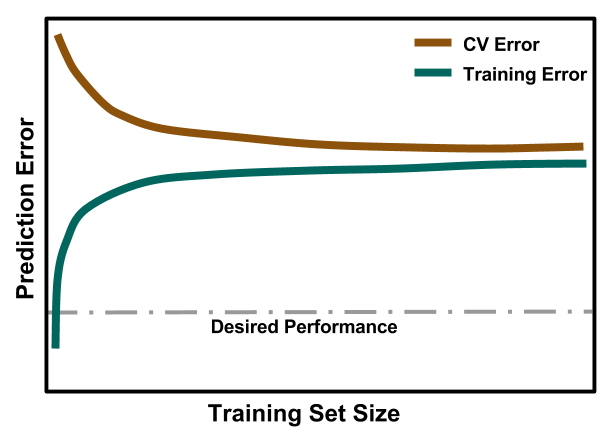
\includegraphics[width=\linewidth]{./figures/LearningCurve-bias.png}
      \caption{High bias and low variance}
    \end{subfigure}%
    \begin{subfigure}{0.33\textwidth}
      \raggedleft
      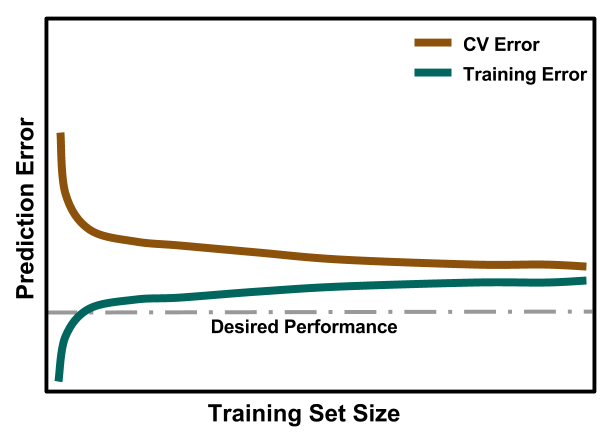
\includegraphics[width=\linewidth]{./figures/LearningCurve-ideal.png}
      \caption{Balanced bias and variance}
    \end{subfigure}%
    \begin{subfigure}{0.33\textwidth}
      \raggedleft
      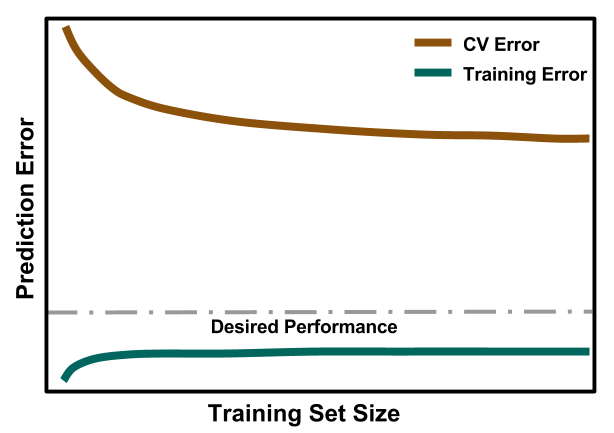
\includegraphics[width=\linewidth]{./figures/LearningCurve-variance.png}
      \caption{Low bias and high variance}
    \end{subfigure}
    \caption{Learning curves for three training scenarios with respect to training set size}
  \end{figure}
\end{frame}

\begin{frame}
  \frametitle{Model Complexity: Validation Curves}
  \begin{figure}[t!]
    \centering
    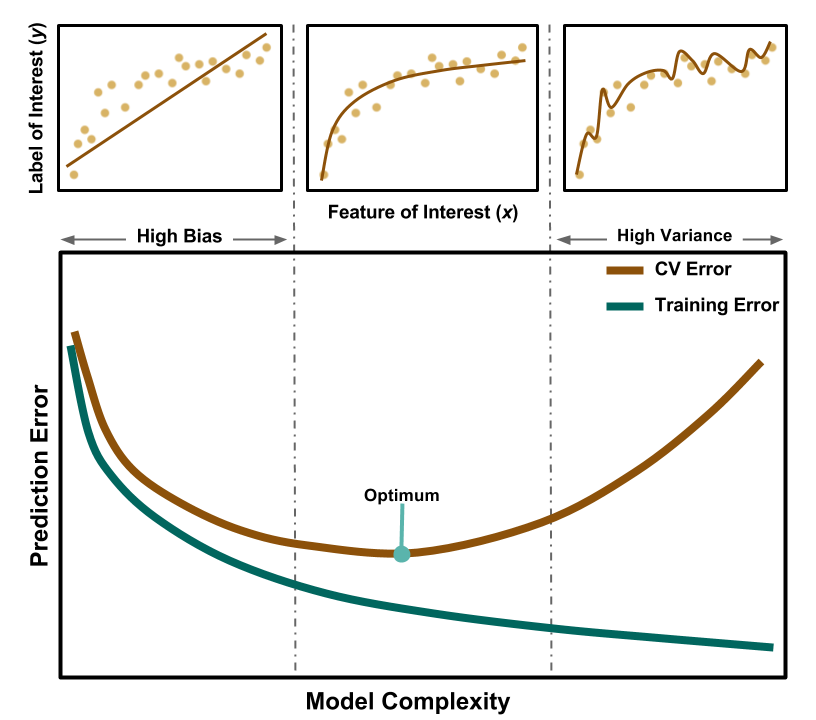
\includegraphics[height=0.75\textheight]{./figures/ValidationCurve.png}
    \caption{Validation curve showing different fitness of models with respect to model complexity}
  \end{figure}
\end{frame}

\begin{frame}
  \frametitle{Model Comparison}
  $$ Posterior = \frac{Likelihood * Prior}{Marginal \ Likelihood} $$
  \begin{table}[h!]
    \centering
    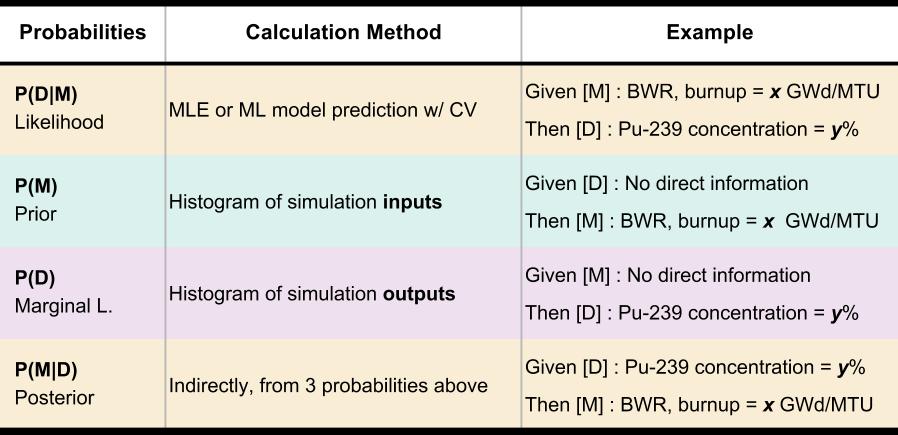
\includegraphics[width=0.8\linewidth]{./figures/bayes.png}
    \caption{Table showing how each component of the model comparison framework will be computed}
  \end{table}
\end{frame}

